%
\chapter{Physical Properties of Low Temperature RF Plasma}\label{sec:chapter_ccrfbasics}
%
	In this first chapter I will provide the necessary physical background for this work about the numerical simulation of low temperature capacitively coupled radio frequency plasmas. Here, both the simulation method as well as the most important aspects about the plasma properties will be introduced.
%
	\section{Plasma Physics}\label{sec:plasmaphysics}
%
  	\subsection{Capacitively Coupled Radio Frequency Plasma}\label{sec:ccrf}
%
		The experiment studied in this work is a capacitively coupled radio frequency discharge with a low temperature plasma, operated at low pressures. Here, I will refer to a plasma as a globally quasi-neutral gas, consisting of freely moving charges --- e.g.\@ electrons, positively and negatively ions --- with additional neutral gas particles. The density ratio between charged and the sum of neutral and charged species defines the \emph{degree of ionization}, which in this case is very low, e.g\@ below 1\%. Charge seperation and violation of quasi-neutrality, which means $n\ix{e}\,=\,n\ix{i}$, is only possible for distances below the \emph{Debye length} $\lambda\ix{D}$.\\
		The creation of a plasma is accomplished by two parallel metal electrodes, where on at least one an ac signal at radio frequency is applied. In the experiment a rf signal at $\SI{13.56}{\mega\hertz}$ with an amplitude between $100$--$\unit[1000]{V}$ is used. This results in a wavelength of $\SI{22.11}{\metre}$ for the electric field wave, which is orders of magnitude larger than the size of the experiment, which is usually below $\SI{10}{\centi\metre}$. Many different electric setups are possible, such as coated or grounded electrodes, producing different operational regimes. Such a system resembles a dielectric hindered plate capacitor. This simplification can be used to understand important physical properties, such as an additional voltage offset on one of the electrodes or charge currents. A basic scheme of an asymmetric rf discharge can be seen in~\autoref{fig:circuitselfbias_1}. For example, non-biased metal surfaces accumulate a negative potential due to the seperation and higher mobility of the electrons. The same goes for electrodes with negative potential and grounded walls. Because continuity has to be satisfied, e.g\@ electron current onto the wall equals ion current, the spatially restricted area of the \emph{plasma sheath} is established.\newpage
%		
		\begin{wrapfigure}[16]{r}{0.42\textwidth}
			\centering
			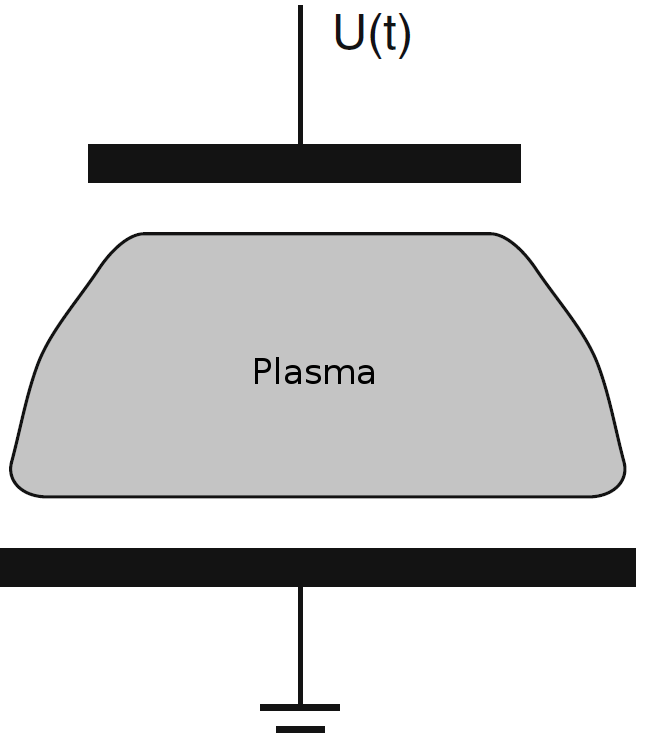
\includegraphics[width=0.38\textwidth]{figures/circuitselfbias_1.png}
			\caption{%
				Schematic of an asymmetric discharge with one grounded and %
			one driven electrode~\cite{Piel10}.}\label{fig:circuitselfbias_1}
		\end{wrapfigure}
%
		 Because continuity has to be satisfied, e.g\@ electron current onto the wall equals ion current, the spatially restricted area of the \emph{plasma sheath} is established. Inside this sheath the electron density drops exponentially towards the wall, where as the ions are accelerated to \emph{Bohm velocity} (see~\autoref{sec:bohmcriteria}). In the case of different electrode sizes the potential inside the sheath can change drastically. If the discharge is driven at radio frequency and an additional capacitance is placed between electrode and generator, the fast charge exchange of electrodes and plasma volume during the collapse of the sheath creates a dc voltage offset, because the capacitor can not be discharged quickly enough. This is called \emph{self bias} (see~\autoref{sec:selfbias}). A displacement current between plasma sheath and volume accommodates as a result of the different time scales of particle movement (see~\autoref{sec:displacementcurrent}). Especially, self-bias and displacement current play a key role in the following investigations, as a capacitive coupling between electrodes and power supply is difficult to model in a numerical kinetic simulation. Radio frequency plasmas are characterized by their unique transport process inside the sheath and heating mechanisms of charged species. A more in-depth discussion can be found in~\autoref{sec:heating}.
